\documentclass[14pt]{extarticle}
\usepackage{amsmath}
\usepackage{amssymb}
\usepackage{graphicx}
\usepackage{tikz}
\usetikzlibrary{calc}
%\usetikzlibrary{trees}
\usepackage{graphicx}
\graphicspath{ {../../chap04/} }
\usepackage[top=0.75in, bottom=0.75in, left=0.75in, right=0.75in]{geometry}
\newcommand*{\Scale}[2][4]{\scalebox{#1}{\ensuremath{#2}}}%
\usepackage[shortlabels]{enumitem}
% \usepackage{showframe}
\title{\vspace{-5ex}Math 208 Section 4.5}
\date{\vspace{-10ex}}
\usepackage{multicol}
\setlength{\columnsep}{1cm}
\newcommand{\tikzmark}[1]{\tikz[overlay,remember picture] \node (#1) {};}
\newcommand{\DrawBox}[4][]{%
	\tikz[overlay,remember picture]{%
		\coordinate (TopLeft)     at ($(#2)+(-0.2em,0.9em)$);
		\coordinate (BottomRight) at ($(#3)+(0.2em,-0.3em)$);
		%
		\path (TopLeft); \pgfgetlastxy{\XCoord}{\IgnoreCoord};
		\path (BottomRight); \pgfgetlastxy{\IgnoreCoord}{\YCoord};
		\coordinate (LabelPoint) at ($(\XCoord,\YCoord)!0.5!(BottomRight)$);
		%
		\draw [red,#1] (TopLeft) rectangle (BottomRight);
		\node [below, #1, fill=none, fill opacity=1] at (LabelPoint) {#4};
	}
}

\begin{document}
\maketitle		
\section*{Homework, Reading, and Other}
\begin{itemize}
	\item Section 4.5
	\item Section 4.6
	\item Exam 1
\end{itemize}

\section*{Goals}
\begin{itemize}
	\item Identify, create, and manipulate \textit{matrix equations}.
	\item Recall and apply the \textit{Basic Properties of Matrices}.
	\item Solve matrix equations of up to thee variables.
\end{itemize}

\section*{4.6 Matrix Equations}
A \textit{Matrix Equation} extends our use of algebra to more easily solve large systems of equations.
\\\\
You already know how to solve $ax=b$ for $x$.
\begin{align*}
	a^{-1}ax &= a^{-1}b \\
	&\text{ which is the same as }\\
	\frac{1}{a}ax &= \frac{1}{a}b \\
	\frac{a}{a}x &= a^{-1}b \\
	x &= a^{-1}b
\end{align*}
Recall from augmented matrices:
\begin{align*}
	&\begin{array}{cc}
		x_1 & x_2 \\
		\downarrow & \downarrow
	\end{array} \\
	&\begin{bmatrix}
		1 & 2 & | & b_1 \\
		3 & 4 & | & b_2
	\end{bmatrix} \to
	\begin{array}{c}
		1x_1+2x_2 = b_1 \\
		3x_1 + 4x_2 = b_2
	\end{array}
\end{align*}
In a matrix equation, we have $AX=B$. Notice:
\begin{align*}
	&\begin{bmatrix}
		1 & 2 \\
		3 & 4
	\end{bmatrix}
	&\begin{bmatrix}
		x_1 \\
		x_2
	\end{bmatrix}
	&=
	&\begin{bmatrix}
		1x_1+2x_2 \\
		3x_1 + 4x_2
	\end{bmatrix} \\
	&2\times 2 &2\times 1 & &2\times 1
\end{align*}
Now we are able to use the \textit{Basic Properties of Matrices} (page 236) to solve matrix equations.\\
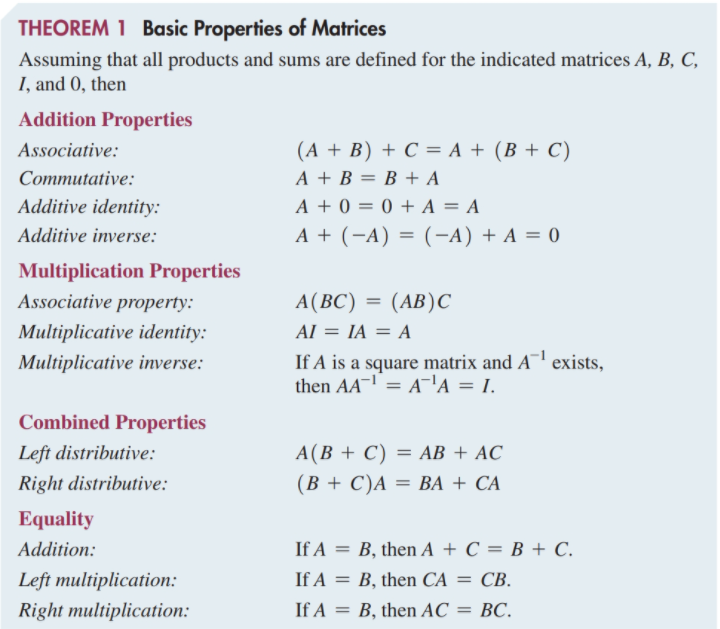
\includegraphics[width=1.0\linewidth]{4-6-1}

\subsection{Solving a Matrix Equation}
\begin{align*}
	AX&=B \\
	A^{-1}AX &=A^{-1}B \tag{ Note that this does not equal $BA^{-1}$} \\
	IX &= A^{-1}B \\
	X &= A^{-1}B
\end{align*}

\subsection{Examples}
\subsubsection{$AX+C=B$}
\begin{align*}
	AX &= B-C \\
	A^{-1}AX &= A^{-1}(B-C)\\
	IX &= A^{-1}(B-C) \\
	X &= A^{-1}(B-C)
\end{align*}

\subsubsection{Solve the system}
\begin{align*}
	\begin{array}{cccc}
		3x_1 - & x_2 + & x_3 & = 1 \\
		-x_1 + & x_2 & & =3 \\
		x_1  & + & x_3 & =2
	\end{array} 
\end{align*}
\begin{align*}
	AX&=B \\
	\begin{bmatrix}
		3 & -1 & 1 \\
		-1 & 1 & 0 \\
		1 & 0 & 1
	\end{bmatrix}
	\begin{bmatrix}	x_1 \\	x_2 \\	x_3	\end{bmatrix}
	&= \begin{bmatrix}	1 \\3 \\2\end{bmatrix}
\end{align*}
So, we need to find $A^{-1}$.
\begin{align*}
	\begin{bmatrix}
		-3 & -1 & 1 & | & 1 & 0 & 0 \\
		-1 & 1 & 0 & | & 0 & 1 & 0 \\
		1 & 0 & 1 & | & 0 & 0 & 1
	\end{bmatrix} \to
	\begin{array}{r}
		R3 \\
		R3+R2 \\
		3R2 + R1
	\end{array}
	\begin{bmatrix}
		1 & 0 & 1 & | & 0 & 0 & 1 \\
		0 & 1 & 1 & | & 0 & 1 & 1 \\
		0 & 2 & 1 & | & 1 & 3 & 0
	\end{bmatrix} \to \\
	\begin{array}{r}
		R1 \\
		R2 \\
		2R2 + R3
	\end{array}
	\begin{bmatrix}
		1 & 0 & 1 & | & 0 & 0 & 1 \\
		0 & 1 & 1 & | & 0 & 1 & 1 \\
		0 & 0 & -1 & | & 1 & 1 & -2
	\end{bmatrix} \to
	\begin{array}{r}
		R3+R1 \\
		R3+R2 \\
		-R3
	\end{array}
	\begin{bmatrix}
		1 & 0 & 0 & | & 1 & 1 & -1 \\
		0 & 1 & 0 & | & 1 & 2 & -1 \\
		0 & 0 & 1 & | & -1 & -1 & 2
	\end{bmatrix}
\end{align*}
and
\begin{align*}
	A^{-1} = \begin{bmatrix}
		1 & 1 & -1 \\
		1 & 2 & -1 \\
		-1 & -1 & 2
	\end{bmatrix}
\end{align*}
Now
\begin{align*}
	AX&=B \\
	X &=A^{-1}B \\
	&= \begin{bmatrix}
		1 & 1 & -1 \\
		1 & 2 & -1 \\
		-1 & -1 & 2
	\end{bmatrix}
	\begin{bmatrix}	1 \\3 \\2\end{bmatrix}
\end{align*}
A $3\times 3$ and a $3\times 1$, so the output is a $3 \times 1$.
\begin{align*}
	X &= \begin{bmatrix}
		1+3-2 \\
		1+6-2 \\
		-1-3+4
	\end{bmatrix}
	= \begin{bmatrix}	x_1=2 \\	x_2=5 \\ x_3=0	\end{bmatrix}
\end{align*}

\subsubsection{Solve the system}
\begin{align*}
	\begin{array}{ccc}
		-2x_1 + & 4x_2 & = -5 \\
		6x_1 - & 12x_2 & = 15
	\end{array}
\end{align*}
\begin{align*}
	A &= \begin{bmatrix}-2 & 4 \\	6 & -12	\end{bmatrix} \\
	A^{-1} &= \frac{1}{24-24} \begin{bmatrix}2 & 6 \\ 4 & 12	\end{bmatrix}
\end{align*}
$A^{-1}$ does not exist, therefore we must solve using augmented Gauss-Jordan.
\begin{align*}
	\begin{bmatrix}
		-2 & 4 & | & -5 \\
		6 & -12 & | & 15
	\end{bmatrix} \to
	\begin{array}{r}
		-\frac{1}{2}R1 \\
		3R1+R2
	\end{array}
	\begin{bmatrix}
		1 & -2 & | & 5/2 \\
		0 & 0 & | & 0
	\end{bmatrix}
\end{align*}
Noting the bottom row, we know we have infinite solutions. Therefore let $x_2=t$, then
\begin{align*}
	x_1-2t &= 5/2 \\
	x_1 &= 2t + 5/2 \\
	x_2 &= t
\end{align*}

\subsubsection{Solve}
\begin{align*}
	\begin{bmatrix}	2 & 6 \\ -4 & -12 \end{bmatrix}
	\begin{bmatrix}	x_1 \\	x_2	\end{bmatrix}
	+ \begin{bmatrix} 5 \\ 2 \end{bmatrix}
	&= \begin{bmatrix} 14 \\ 7 \end{bmatrix} \\
	\begin{bmatrix}	2 & 6 \\ -4 & -12 \end{bmatrix}
	\begin{bmatrix}	x_1 \\	x_2	\end{bmatrix}
	&= \begin{bmatrix} 14-5 \\ 7-2 \end{bmatrix}
	= \begin{bmatrix} 9 \\ 5 \end{bmatrix}
\end{align*}
Just like the previous example, $A^{-1}$ does not exist and we need to use G-J.
\begin{align*}
	\begin{bmatrix}	2 & 6 & | & 9 \\
		-4 & -12 & | & 5 \end{bmatrix} \to
	\begin{array}{r}
		\frac{1}{2}R1 \\
		2R1+R2
	\end{array}
	\begin{bmatrix}	1 & 3 & | & 9/2 \\
		0 & 0 & | & 23 \end{bmatrix}
\end{align*}
Noting the bottom row, we know we have no solution!

\subsubsection{$AX + BX =C$}
\begin{align*}
	(A+B)X &=C \\
	(A+B)^{-1}(A+B)X &=(A+B)^{-1}C \\
	IX &=(A+B)^{-1}C \\
	X &=(A+B)^{-1}C
\end{align*}

\subsubsection{Solve}
\begin{align*}
	\begin{bmatrix}
		5 & 10 \\
		4 & 7
	\end{bmatrix}
	\begin{bmatrix}
		x_1 \\
		x_2
	\end{bmatrix}
	- \begin{bmatrix}
		2 & -1 \\
		3 & 3
	\end{bmatrix}
	\begin{bmatrix}
		x_1 \\
		x_2
	\end{bmatrix}
	&= \begin{bmatrix} 97 \\ 35 \end{bmatrix}	
\end{align*}
Similar to the previous example.
\begin{align*}
	\left(
	\begin{bmatrix}
		5 & 10 \\
		4 & 7
	\end{bmatrix}
	- \begin{bmatrix}
		2 & -1 \\
		3 & 3
	\end{bmatrix}
	\right)
	\begin{bmatrix}
		x_1 \\
		x_2
	\end{bmatrix}
	&= \begin{bmatrix} 97 \\ 35 \end{bmatrix} \\
	\begin{bmatrix}
		3 & 11 \\
		1 & 4
	\end{bmatrix}
	\begin{bmatrix}
		x_1 \\
		x_2
	\end{bmatrix}
	&= \begin{bmatrix} 97 \\ 35 \end{bmatrix}
\end{align*}
Find the inverse
\begin{align*}
	\begin{bmatrix}
		3 & 11 \\
		1 & 4
	\end{bmatrix}^{-1}
	= \frac{1}{12-11}\begin{bmatrix}
		4 & -11 \\
		-1 & 3
	\end{bmatrix}
	= \begin{bmatrix}
		4 & -11 \\
		-1 & 3
	\end{bmatrix}
\end{align*}
and solve
\begin{align*}
	\begin{bmatrix}
		x_1 \\
		x_2
	\end{bmatrix}
	= \begin{bmatrix}
		4 & -11 \\
		-1 & 3
	\end{bmatrix}\begin{bmatrix} 97 \\ 35 \end{bmatrix}
	= \begin{bmatrix} 388-385 \\ -97+105 \end{bmatrix}
	= \begin{bmatrix} 3 \\ 8 \end{bmatrix}
\end{align*}


\cleardoublepage


\end{document}
